\chapter{CEMicro Implementation}
\label{sec:impl}


\section{Setting up the Development Environment}

- Visual Studio Code (code editor) https://code.visualstudio.com/

- Git (version control) https://git-scm.com/

- Virtualisation with Docker

- Node.js

Challenge: Setting up git/bash on windows

Challenge: File permissions for docker on windows


\section{Application Programming Interfaces}

- REST

- Swagger/OpenApi

- Single source of truth

Discarded: Saving Templates in CEMicro (see single source of truth page)

Discarded: swagger-tools

\begin{figure}
  \centering
  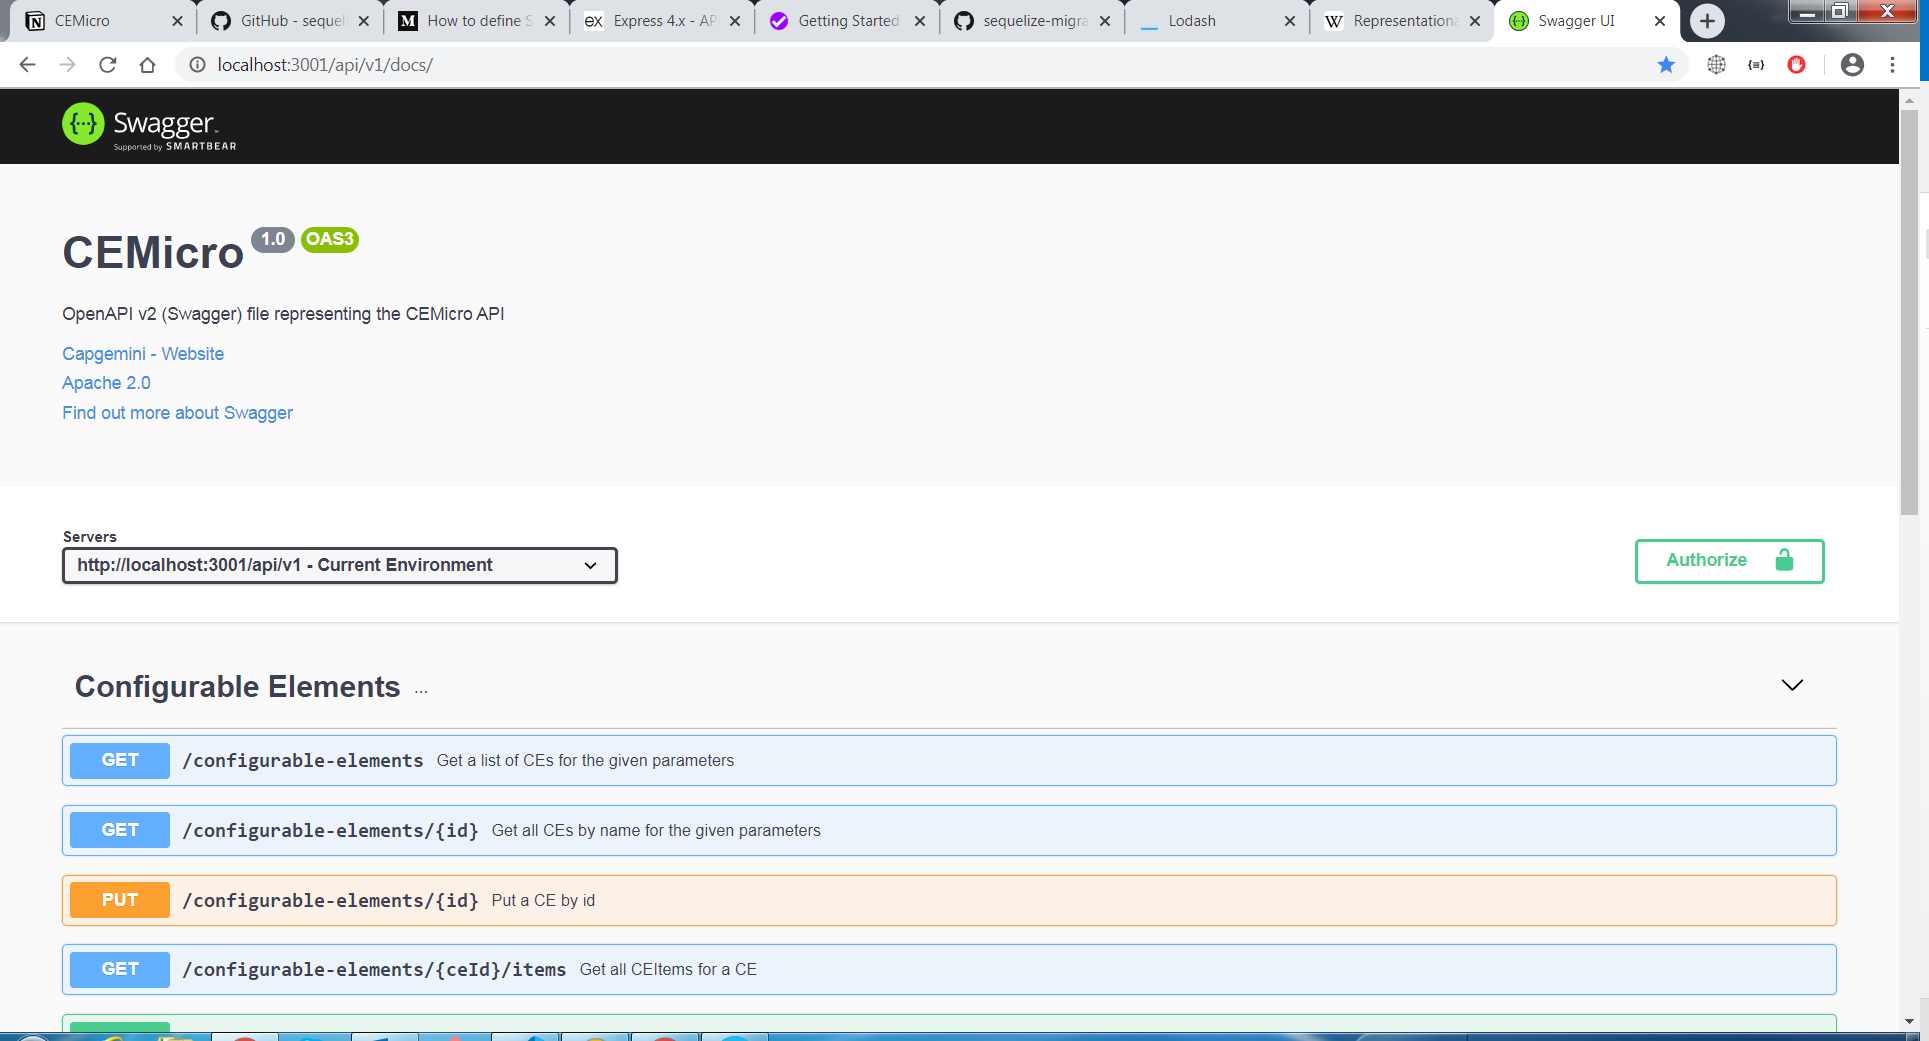
\includegraphics[width=0.8\linewidth]{assets/swagger-api-docs.png}
  \caption{Interactive API documentation with Swagger}
  \label{fig:api-docs}
\end{figure}


\section{Backend Framework with Express.js}

Tools:

Nodemon

Express

Express Validator

MVC -> MVCS (Model View Controller Service)


\section{Data persistance with PosgreSQL}

Sequelize

https://github.com/sequelize/express-example

Discarded: Flyway-db, Umzug

Migrations: Sequelize


\section{Frontend Framework with Vue.js}

To do ...


\section{Virtualisation with Docker}

- install packages, build, prune packages


\section{Interfacing with the monolith development team}

Changes to Docify


\section{Challanges during development}

- Knowing how to set up the development environment

- Understanding the task, see [CE Properties](https://www.notion.so/CE-Properties-7bf08f28c69344c1957e7072c1101fd6)

- Setting up git/bash on windows

- File permissions for docker on windows ([https://medium.com/@akash1233/change-file-permissions-when-working-with-git-repos-on-windows-ea22e34d5cee](https://medium.com/@akash1233/change-file-permissions-when-working-with-git-repos-on-windows-ea22e34d5cee))


\section{Documentation of CEMicro}

Providing a foundation for others to build on (Confluence, Readme, Thesis)
